% Options for packages loaded elsewhere
\PassOptionsToPackage{unicode}{hyperref}
\PassOptionsToPackage{hyphens}{url}
\documentclass[
]{article}
\usepackage{xcolor}
\usepackage[margin=1in]{geometry}
\usepackage{amsmath,amssymb}
\setcounter{secnumdepth}{5}
\usepackage{iftex}
\ifPDFTeX
  \usepackage[T1]{fontenc}
  \usepackage[utf8]{inputenc}
  \usepackage{textcomp} % provide euro and other symbols
\else % if luatex or xetex
  \usepackage{unicode-math} % this also loads fontspec
  \defaultfontfeatures{Scale=MatchLowercase}
  \defaultfontfeatures[\rmfamily]{Ligatures=TeX,Scale=1}
\fi
\usepackage{lmodern}
\ifPDFTeX\else
  % xetex/luatex font selection
\fi
% Use upquote if available, for straight quotes in verbatim environments
\IfFileExists{upquote.sty}{\usepackage{upquote}}{}
\IfFileExists{microtype.sty}{% use microtype if available
  \usepackage[]{microtype}
  \UseMicrotypeSet[protrusion]{basicmath} % disable protrusion for tt fonts
}{}
\makeatletter
\@ifundefined{KOMAClassName}{% if non-KOMA class
  \IfFileExists{parskip.sty}{%
    \usepackage{parskip}
  }{% else
    \setlength{\parindent}{0pt}
    \setlength{\parskip}{6pt plus 2pt minus 1pt}}
}{% if KOMA class
  \KOMAoptions{parskip=half}}
\makeatother
\usepackage{color}
\usepackage{fancyvrb}
\newcommand{\VerbBar}{|}
\newcommand{\VERB}{\Verb[commandchars=\\\{\}]}
\DefineVerbatimEnvironment{Highlighting}{Verbatim}{commandchars=\\\{\}}
% Add ',fontsize=\small' for more characters per line
\usepackage{framed}
\definecolor{shadecolor}{RGB}{248,248,248}
\newenvironment{Shaded}{\begin{snugshade}}{\end{snugshade}}
\newcommand{\AlertTok}[1]{\textcolor[rgb]{0.94,0.16,0.16}{#1}}
\newcommand{\AnnotationTok}[1]{\textcolor[rgb]{0.56,0.35,0.01}{\textbf{\textit{#1}}}}
\newcommand{\AttributeTok}[1]{\textcolor[rgb]{0.13,0.29,0.53}{#1}}
\newcommand{\BaseNTok}[1]{\textcolor[rgb]{0.00,0.00,0.81}{#1}}
\newcommand{\BuiltInTok}[1]{#1}
\newcommand{\CharTok}[1]{\textcolor[rgb]{0.31,0.60,0.02}{#1}}
\newcommand{\CommentTok}[1]{\textcolor[rgb]{0.56,0.35,0.01}{\textit{#1}}}
\newcommand{\CommentVarTok}[1]{\textcolor[rgb]{0.56,0.35,0.01}{\textbf{\textit{#1}}}}
\newcommand{\ConstantTok}[1]{\textcolor[rgb]{0.56,0.35,0.01}{#1}}
\newcommand{\ControlFlowTok}[1]{\textcolor[rgb]{0.13,0.29,0.53}{\textbf{#1}}}
\newcommand{\DataTypeTok}[1]{\textcolor[rgb]{0.13,0.29,0.53}{#1}}
\newcommand{\DecValTok}[1]{\textcolor[rgb]{0.00,0.00,0.81}{#1}}
\newcommand{\DocumentationTok}[1]{\textcolor[rgb]{0.56,0.35,0.01}{\textbf{\textit{#1}}}}
\newcommand{\ErrorTok}[1]{\textcolor[rgb]{0.64,0.00,0.00}{\textbf{#1}}}
\newcommand{\ExtensionTok}[1]{#1}
\newcommand{\FloatTok}[1]{\textcolor[rgb]{0.00,0.00,0.81}{#1}}
\newcommand{\FunctionTok}[1]{\textcolor[rgb]{0.13,0.29,0.53}{\textbf{#1}}}
\newcommand{\ImportTok}[1]{#1}
\newcommand{\InformationTok}[1]{\textcolor[rgb]{0.56,0.35,0.01}{\textbf{\textit{#1}}}}
\newcommand{\KeywordTok}[1]{\textcolor[rgb]{0.13,0.29,0.53}{\textbf{#1}}}
\newcommand{\NormalTok}[1]{#1}
\newcommand{\OperatorTok}[1]{\textcolor[rgb]{0.81,0.36,0.00}{\textbf{#1}}}
\newcommand{\OtherTok}[1]{\textcolor[rgb]{0.56,0.35,0.01}{#1}}
\newcommand{\PreprocessorTok}[1]{\textcolor[rgb]{0.56,0.35,0.01}{\textit{#1}}}
\newcommand{\RegionMarkerTok}[1]{#1}
\newcommand{\SpecialCharTok}[1]{\textcolor[rgb]{0.81,0.36,0.00}{\textbf{#1}}}
\newcommand{\SpecialStringTok}[1]{\textcolor[rgb]{0.31,0.60,0.02}{#1}}
\newcommand{\StringTok}[1]{\textcolor[rgb]{0.31,0.60,0.02}{#1}}
\newcommand{\VariableTok}[1]{\textcolor[rgb]{0.00,0.00,0.00}{#1}}
\newcommand{\VerbatimStringTok}[1]{\textcolor[rgb]{0.31,0.60,0.02}{#1}}
\newcommand{\WarningTok}[1]{\textcolor[rgb]{0.56,0.35,0.01}{\textbf{\textit{#1}}}}
\usepackage{longtable,booktabs,array}
\usepackage{calc} % for calculating minipage widths
% Correct order of tables after \paragraph or \subparagraph
\usepackage{etoolbox}
\makeatletter
\patchcmd\longtable{\par}{\if@noskipsec\mbox{}\fi\par}{}{}
\makeatother
% Allow footnotes in longtable head/foot
\IfFileExists{footnotehyper.sty}{\usepackage{footnotehyper}}{\usepackage{footnote}}
\makesavenoteenv{longtable}
\usepackage{graphicx}
\makeatletter
\newsavebox\pandoc@box
\newcommand*\pandocbounded[1]{% scales image to fit in text height/width
  \sbox\pandoc@box{#1}%
  \Gscale@div\@tempa{\textheight}{\dimexpr\ht\pandoc@box+\dp\pandoc@box\relax}%
  \Gscale@div\@tempb{\linewidth}{\wd\pandoc@box}%
  \ifdim\@tempb\p@<\@tempa\p@\let\@tempa\@tempb\fi% select the smaller of both
  \ifdim\@tempa\p@<\p@\scalebox{\@tempa}{\usebox\pandoc@box}%
  \else\usebox{\pandoc@box}%
  \fi%
}
% Set default figure placement to htbp
\def\fps@figure{htbp}
\makeatother
\setlength{\emergencystretch}{3em} % prevent overfull lines
\providecommand{\tightlist}{%
  \setlength{\itemsep}{0pt}\setlength{\parskip}{0pt}}
\usepackage{booktabs}
\usepackage{longtable}
\usepackage{array}
\usepackage{multirow}
\usepackage{wrapfig}
\usepackage{float}
\usepackage{colortbl}
\usepackage{pdflscape}
\usepackage{tabu}
\usepackage{threeparttable}
\usepackage{threeparttablex}
\usepackage[normalem]{ulem}
\usepackage{makecell}
\usepackage{xcolor}
\usepackage{bookmark}
\IfFileExists{xurl.sty}{\usepackage{xurl}}{} % add URL line breaks if available
\urlstyle{same}
\hypersetup{
  pdftitle={Forecast of the USD/CNY Exchange Rate on April 16, 2025},
  pdfauthor={Iushin Nikolai},
  pdfsubject={International Finance},
  hidelinks,
  pdfcreator={LaTeX via pandoc}}

\title{Forecast of the USD/CNY Exchange Rate on April 16, 2025}
\author{Iushin Nikolai}
\date{2025-04-08}

\begin{document}
\maketitle

{
\setcounter{tocdepth}{2}
\tableofcontents
}
\subsection{Objective}\label{objective}

The purpose of this report is to forecast the bilateral nominal exchange
rate between the Chinese renminbi (CNY) and the U.S. dollar (USD) on
\textbf{April 16, 2025}, utilizing a range of theoretical models
grounded in international finance.

The following models are employed to produce the forecast:

\begin{itemize}
\item
  \textbf{Uncovered Interest Parity (UIP):} A theory stating that the
  difference in interest rates between two countries will be reflected
  in future changes in the exchange rate. Investors are assumed to be
  risk-neutral and indifferent between domestic and foreign assets,
  expecting equal returns once adjusted for exchange rate movements.
\item
  \textbf{Covered Interest Parity (CIP):} A no-arbitrage condition in
  which the forward exchange rate eliminates any profit opportunity from
  interest rate differentials. It assumes the availability of forward
  contracts to hedge exchange rate risk completely.
\item
  \textbf{Forward Premium Approach:} This approach uses the proportional
  difference between forward and spot exchange rates (forward premium or
  discount) as a predictor of expected depreciation or appreciation,
  under the assumption that forward rates are unbiased predictors of
  future spot rates.
\item
  \textbf{Historical Trend (ARIMA):} A purely time-series-based
  statistical model---AutoRegressive Integrated Moving Average---is
  applied to capture historical dynamics and forecast future values of
  the USD/CNY rate based on past behavior, without requiring
  macroeconomic fundamentals.
\end{itemize}

\subsection{Data Source: Yahoo Finance}\label{data-source-yahoo-finance}

Exchange rate data are retrieved from \textbf{Yahoo Finance},
specifically the time series for the USD/CNY spot exchange rate
(\texttt{CNY=X}). The data covers the period from January 2024 to April
2025. The spot exchange rate observed on \textbf{April 7, 2025} (7.1679)
is used as the baseline input for theoretical models.

Additionally, interest rate estimates are extracted from publicly
available macroeconomic sources:

\begin{itemize}
\tightlist
\item
  \textbf{U.S. Federal Funds Rate (i\_USD):} 4.33\%
\item
  \textbf{People's Bank of China Benchmark Lending Rate (i\_CNY):}
  3.10\%
\end{itemize}

These rates represent the annualized short-term nominal interest rates
and are used to compute expected exchange rate changes over a two-month
horizon.

\begin{Shaded}
\begin{Highlighting}[]
\FunctionTok{library}\NormalTok{(quantmod)}
\end{Highlighting}
\end{Shaded}

\begin{verbatim}
## Loading required package: xts
\end{verbatim}

\begin{verbatim}
## Loading required package: zoo
\end{verbatim}

\begin{verbatim}
## 
## Attaching package: 'zoo'
\end{verbatim}

\begin{verbatim}
## The following objects are masked from 'package:base':
## 
##     as.Date, as.Date.numeric
\end{verbatim}

\begin{verbatim}
## Loading required package: TTR
\end{verbatim}

\begin{verbatim}
## Registered S3 method overwritten by 'quantmod':
##   method            from
##   as.zoo.data.frame zoo
\end{verbatim}

\begin{Shaded}
\begin{Highlighting}[]
\FunctionTok{library}\NormalTok{(tidyverse)}
\end{Highlighting}
\end{Shaded}

\begin{verbatim}
## -- Attaching core tidyverse packages ------------------------ tidyverse 2.0.0 --
## v dplyr     1.1.4     v readr     2.1.5
## v forcats   1.0.0     v stringr   1.5.1
## v ggplot2   3.5.1     v tibble    3.2.1
## v lubridate 1.9.4     v tidyr     1.3.1
## v purrr     1.0.4
\end{verbatim}

\begin{verbatim}
## -- Conflicts ------------------------------------------ tidyverse_conflicts() --
## x dplyr::filter() masks stats::filter()
## x dplyr::first()  masks xts::first()
## x dplyr::lag()    masks stats::lag()
## x dplyr::last()   masks xts::last()
## i Use the conflicted package (<http://conflicted.r-lib.org/>) to force all conflicts to become errors
\end{verbatim}

\begin{Shaded}
\begin{Highlighting}[]
\FunctionTok{library}\NormalTok{(tidyquant)}
\end{Highlighting}
\end{Shaded}

\begin{verbatim}
## -- Attaching core tidyquant packages ----------------------- tidyquant 1.0.11 --
## v PerformanceAnalytics 2.0.8     
## -- Conflicts ------------------------------------------ tidyquant_conflicts() --
## x zoo::as.Date()                 masks base::as.Date()
## x zoo::as.Date.numeric()         masks base::as.Date.numeric()
## x dplyr::filter()                masks stats::filter()
## x dplyr::first()                 masks xts::first()
## x dplyr::lag()                   masks stats::lag()
## x dplyr::last()                  masks xts::last()
## x PerformanceAnalytics::legend() masks graphics::legend()
## x quantmod::summary()            masks base::summary()
## i Use the conflicted package (<http://conflicted.r-lib.org/>) to force all conflicts to become errors
\end{verbatim}

\begin{Shaded}
\begin{Highlighting}[]
\FunctionTok{library}\NormalTok{(lubridate)}
\FunctionTok{library}\NormalTok{(forecast)}
\FunctionTok{library}\NormalTok{(kableExtra)}
\end{Highlighting}
\end{Shaded}

\begin{verbatim}
## 
## Attaching package: 'kableExtra'
## 
## The following object is masked from 'package:dplyr':
## 
##     group_rows
\end{verbatim}

\begin{Shaded}
\begin{Highlighting}[]
\FunctionTok{library}\NormalTok{(rvest)}
\end{Highlighting}
\end{Shaded}

\begin{verbatim}
## 
## Attaching package: 'rvest'
## 
## The following object is masked from 'package:readr':
## 
##     guess_encoding
\end{verbatim}

\begin{Shaded}
\begin{Highlighting}[]
\FunctionTok{library}\NormalTok{(stringr)}
\FunctionTok{library}\NormalTok{(tibble)}
\FunctionTok{library}\NormalTok{(knitr)}
\end{Highlighting}
\end{Shaded}

\subsection{Initial Data}\label{initial-data}

To forecast the USD/CNY exchange rate on April 16, 2025, we collect the
necessary economic and market inputs as follows:

\begin{itemize}
\item
  \textbf{Spot Exchange Rate (USD/CNY):} The spot rate as of April 7,
  2025, is retrieved from Yahoo Finance using the ticker \texttt{CNY=X}.
  The closing exchange rate on this date is \textbf{7.253}. This rate
  serves as the current nominal bilateral exchange rate to be used in
  theoretical models such as UIP and CIP.
\item
  \textbf{U.S. Interest Rate (i\_USD):} The effective federal funds rate
  is obtained from the Federal Reserve Economic Data (FRED) via the
  \texttt{FEDFUNDS} series. We extract the latest available rate as of
  April 7, 2025, which is \textbf{4.33\%} (i.e.,
  \texttt{i\_usd\ =\ 0.0433} in decimal form).
\item
  \textbf{China's Interest Rate (i\_CNY):} The benchmark lending rate is
  retrieved through web scraping from
  \href{https://tradingeconomics.com/china/interest-rate}{TradingEconomics},
  a reputable source for macroeconomic indicators. The most recent rate
  available is \textbf{3.10\%} (i.e., \texttt{i\_cny\ =\ 0.031} in
  decimal form).
\item
  \textbf{Forecast Horizon:} Since the target date is exactly
  \textbf{one week} ahead of the spot rate observation date, we define
  the forecast horizon as \(\frac{1}{52}\) years (i.e.,
  \texttt{horizon\ =\ 1/52}), assuming 52 weeks in a year. This
  short-term window is particularly appropriate for models like UIP and
  CIP, which are sensitive to interest rate differentials even over
  brief periods.
\end{itemize}

\begin{Shaded}
\begin{Highlighting}[]
\CommentTok{\# Spot Exchange Rate (USD/CNY)}
\FunctionTok{getSymbols}\NormalTok{(}\StringTok{"CNY=X"}\NormalTok{, }\AttributeTok{src =} \StringTok{"yahoo"}\NormalTok{, }\AttributeTok{from =} \StringTok{"2024{-}01{-}01"}\NormalTok{, }\AttributeTok{to =} \StringTok{"2025{-}04{-}07"}\NormalTok{)}
\end{Highlighting}
\end{Shaded}

\begin{verbatim}
## Warning: CNY=X contains missing values. Some functions will not work if objects
## contain missing values in the middle of the series. Consider using na.omit(),
## na.approx(), na.fill(), etc to remove or replace them.
\end{verbatim}

\begin{verbatim}
## [1] "CNY=X"
\end{verbatim}

\begin{Shaded}
\begin{Highlighting}[]
\NormalTok{fx\_data }\OtherTok{\textless{}{-}} \StringTok{\textasciigrave{}}\AttributeTok{CNY=X}\StringTok{\textasciigrave{}}
\NormalTok{spot\_rate }\OtherTok{\textless{}{-}} \FunctionTok{Cl}\NormalTok{(fx\_data[}\StringTok{"2025{-}04{-}06"}\NormalTok{])}

\CommentTok{\# U.S. Interest Rate (i\_USD)}
\NormalTok{fed\_rate }\OtherTok{\textless{}{-}} \FunctionTok{tq\_get}\NormalTok{(}\StringTok{"FEDFUNDS"}\NormalTok{, }\AttributeTok{get =} \StringTok{"economic.data"}\NormalTok{, }\AttributeTok{from =} \StringTok{"2024{-}01{-}01"}\NormalTok{) }\SpecialCharTok{\%\textgreater{}\%}
  \FunctionTok{filter}\NormalTok{(date }\SpecialCharTok{\textless{}=} \FunctionTok{as.Date}\NormalTok{(}\StringTok{"2025{-}04{-}07"}\NormalTok{)) }\SpecialCharTok{\%\textgreater{}\%}
  \FunctionTok{tail}\NormalTok{(}\DecValTok{1}\NormalTok{) }\SpecialCharTok{\%\textgreater{}\%}
  \FunctionTok{pull}\NormalTok{(price) }\SpecialCharTok{/} \DecValTok{100}  

\NormalTok{i\_usd }\OtherTok{\textless{}{-}}\NormalTok{ fed\_rate}

\CommentTok{\# China’s Interest Rate (i\_CNY)}
\NormalTok{url }\OtherTok{\textless{}{-}} \StringTok{"https://tradingeconomics.com/china/interest{-}rate"}
\NormalTok{page }\OtherTok{\textless{}{-}} \FunctionTok{read\_html}\NormalTok{(url)}
\NormalTok{rate\_node }\OtherTok{\textless{}{-}}\NormalTok{ page }\SpecialCharTok{\%\textgreater{}\%}
  \FunctionTok{html\_elements}\NormalTok{(}\StringTok{"table"}\NormalTok{) }\SpecialCharTok{\%\textgreater{}\%}
  \FunctionTok{html\_text2}\NormalTok{() }\SpecialCharTok{\%\textgreater{}\%}
  \FunctionTok{str\_extract}\NormalTok{(}\StringTok{"}\SpecialCharTok{\textbackslash{}\textbackslash{}}\StringTok{b}\SpecialCharTok{\textbackslash{}\textbackslash{}}\StringTok{d\{1,2\}}\SpecialCharTok{\textbackslash{}\textbackslash{}}\StringTok{.}\SpecialCharTok{\textbackslash{}\textbackslash{}}\StringTok{d\{1,2\}}\SpecialCharTok{\textbackslash{}\textbackslash{}}\StringTok{b"}\NormalTok{) }\SpecialCharTok{\%\textgreater{}\%}
\NormalTok{  .[}\DecValTok{1}\NormalTok{]}
\NormalTok{i\_cny }\OtherTok{\textless{}{-}} \FunctionTok{as.numeric}\NormalTok{(rate\_node) }\SpecialCharTok{/} \DecValTok{100}

\CommentTok{\# Forecast Horizon}
\NormalTok{horizon }\OtherTok{\textless{}{-}} \FloatTok{0.0192}\SpecialCharTok{/}\DecValTok{12}  \CommentTok{\# 1 week}


\NormalTok{input\_table }\OtherTok{\textless{}{-}} \FunctionTok{tibble}\NormalTok{(}
  \AttributeTok{Indicator =} \FunctionTok{c}\NormalTok{(}\StringTok{"Spot Exchange Rate (USD/CNY)"}\NormalTok{, }
                \StringTok{"U.S. Interest Rate (i\_USD)"}\NormalTok{, }
                \StringTok{"China Interest Rate (i\_CNY)"}\NormalTok{, }
                \StringTok{"Forecast Horizon (years)"}\NormalTok{),}
  \AttributeTok{Value =} \FunctionTok{c}\NormalTok{(}\FunctionTok{as.numeric}\NormalTok{(spot\_rate),}
            \FunctionTok{round}\NormalTok{(i\_usd, }\DecValTok{4}\NormalTok{),}
            \FunctionTok{round}\NormalTok{(i\_cny, }\DecValTok{4}\NormalTok{),}
            \FunctionTok{round}\NormalTok{(horizon, }\DecValTok{6}\NormalTok{))}
\NormalTok{)}

\FunctionTok{kable}\NormalTok{(input\_table, }\AttributeTok{caption =} \StringTok{"Summary of Initial Input Variables"}\NormalTok{)}
\end{Highlighting}
\end{Shaded}

\begin{longtable}[]{@{}lr@{}}
\caption{Summary of Initial Input Variables}\tabularnewline
\toprule\noalign{}
Indicator & Value \\
\midrule\noalign{}
\endfirsthead
\toprule\noalign{}
Indicator & Value \\
\midrule\noalign{}
\endhead
\bottomrule\noalign{}
\endlastfoot
Spot Exchange Rate (USD/CNY) & 7.2813 \\
U.S. Interest Rate (i\_USD) & 0.0433 \\
China Interest Rate (i\_CNY) & 0.0310 \\
Forecast Horizon (years) & 0.0016 \\
\end{longtable}

\subsection{Forecast Based on the UIP
Model}\label{forecast-based-on-the-uip-model}

The \textbf{Uncovered Interest Parity (UIP)} model provides a
theoretical framework to predict future spot exchange rates based on
interest rate differentials between two countries. Under the UIP
condition, the expected appreciation or depreciation of a currency is
proportional to the difference between domestic and foreign interest
rates.

The core UIP formula is:

\[
E_{t+h}(S) = S_t \times \left( \frac{1 + i_{\text{domestic}}}{1 + i_{\text{foreign}}} \right)^h
\]

Where:

\begin{itemize}
\tightlist
\item
  \(E_{t+h}(S)\) --- expected future spot exchange rate at horizon
  \(h\)\\
\item
  \(S_t\) --- current spot rate (USD/CNY on April 6, 2025):
  \textbf{7.253}\\
\item
  \(i_{\text{domestic}}\) --- U.S. short-term interest rate:
  \textbf{4.33\%}\\
\item
  \(i_{\text{foreign}}\) --- China's short-term interest rate:
  \textbf{3.10\%}\\
\item
  \(h\) --- time horizon in years (1 week):
  \(h = \frac{1}{52} \approx 0.0192\)
\end{itemize}

\begin{center}\rule{0.5\linewidth}{0.5pt}\end{center}

\subsubsection{Calculation}\label{calculation}

Using the most recent data:

\[
E_{t+1\text{ week}}(USD/CNY) = 7.253 \times \left( \frac{1 + 0.0433}{1 + 0.031} \right)^{0.0192} \approx \mathbf{7.2814}
\]

\begin{Shaded}
\begin{Highlighting}[]
\NormalTok{uip\_forecast }\OtherTok{\textless{}{-}} \FunctionTok{as.numeric}\NormalTok{(spot\_rate) }\SpecialCharTok{*}\NormalTok{ ((}\DecValTok{1} \SpecialCharTok{+}\NormalTok{ i\_usd)}\SpecialCharTok{/}\NormalTok{(}\DecValTok{1} \SpecialCharTok{+}\NormalTok{ i\_cny))}\SpecialCharTok{\^{}}\NormalTok{horizon}
\NormalTok{uip\_forecast}
\end{Highlighting}
\end{Shaded}

\begin{verbatim}
## [1] 7.281438
\end{verbatim}

\begin{center}\rule{0.5\linewidth}{0.5pt}\end{center}

According to the UIP model, the Chinese yuan is expected to
\textbf{depreciate slightly} against the U.S. dollar over the next week.
The predicted exchange rate on \textbf{April 16, 2025} is \textbf{7.2814
USD/CNY}. This modest weakening of the RMB is consistent with the
positive interest rate differential in favor of the U.S. dollar.

\subsection{Forecast Based on the CIP
Model}\label{forecast-based-on-the-cip-model}

The \textbf{Covered Interest Parity (CIP)} model is a foundational
concept in international finance, describing an arbitrage-free condition
between spot and forward exchange rates when hedging via forward
contracts is available. Under CIP, the relationship between spot and
forward exchange rates reflects the interest rate differential between
two countries.

The CIP equation is given by:

\[
F_{t}(S) = S_t \times \left( \frac{1 + i_{\text{domestic}}}{1 + i_{\text{foreign}}} \right)^h
\]

Where:

\begin{itemize}
\tightlist
\item
  \(F_t(S)\) --- forward exchange rate implied by interest parity\\
\item
  \(S_t\) --- spot rate at time \(t\): \textbf{7.253} (USD/CNY on April
  6, 2025)\\
\item
  \(i_{\text{domestic}}\) --- U.S. interest rate: \textbf{4.33\%}\\
\item
  \(i_{\text{foreign}}\) --- China's interest rate: \textbf{3.10\%}\\
\item
  \(h\) --- forecast horizon in years:
  \(h = \frac{1}{52} \approx 0.0192\)
\end{itemize}

\begin{center}\rule{0.5\linewidth}{0.5pt}\end{center}

\subsubsection{Calculation}\label{calculation-1}

\[
F_t(USD/CNY) = 7.253 \times \left( \frac{1 + 0.0433}{1 + 0.031} \right)^{0.0192} \approx \mathbf{7.2814}
\]

\begin{Shaded}
\begin{Highlighting}[]
\NormalTok{cip\_forward\_rate }\OtherTok{\textless{}{-}} \FunctionTok{as.numeric}\NormalTok{(spot\_rate) }\SpecialCharTok{*}\NormalTok{ ((}\DecValTok{1} \SpecialCharTok{+}\NormalTok{ i\_usd) }\SpecialCharTok{/}\NormalTok{ (}\DecValTok{1} \SpecialCharTok{+}\NormalTok{ i\_cny))}\SpecialCharTok{\^{}}\NormalTok{horizon}
\NormalTok{cip\_forward\_rate}
\end{Highlighting}
\end{Shaded}

\begin{verbatim}
## [1] 7.281438
\end{verbatim}

\begin{center}\rule{0.5\linewidth}{0.5pt}\end{center}

\subsubsection{Conclusion}\label{conclusion}

The CIP model implies a \textbf{forward exchange rate of 7.2814 USD/CNY}
for April 16, 2025. This value coincides with the UIP prediction due to
the use of identical inputs. The forward rate reflects the interest rate
advantage of the U.S. dollar and suggests that investors would require a
slightly higher rate of yuan per dollar in the future to prevent
arbitrage opportunities.

\subsection{Forecast Based on ARIMA
Model}\label{forecast-based-on-arima-model}

To account for the time-series dynamics of the USD/CNY exchange rate, we
apply an \textbf{ARIMA model} --- AutoRegressive Integrated Moving
Average --- which is widely used in financial forecasting due to its
ability to capture trends, seasonality, and volatility.

\subsubsection{Model Specification}\label{model-specification}

Using \texttt{auto.arima()} from the \texttt{forecast} package in R, the
best-fitting model is identified as:

\[
\text{ARIMA}(4,1,5)
\]

This model includes: - 4 autoregressive (AR) terms - 1 order of
differencing (I) - 5 moving average (MA) terms

The model is estimated based on daily closing prices of the USD/CNY spot
rate from January 2024 to April 6, 2025.

\begin{center}\rule{0.5\linewidth}{0.5pt}\end{center}

\subsubsection{Forecast Procedure}\label{forecast-procedure}

A 7-day ahead forecast is generated to approximate the expected exchange
rate on \textbf{April 16, 2025}. The predicted value on the 7th
forecasted day is:

\[
\hat{S}_{\text{ARIMA, t+7}} = \mathbf{7.2793}
\]

\begin{center}\rule{0.5\linewidth}{0.5pt}\end{center}

\begin{Shaded}
\begin{Highlighting}[]
\NormalTok{fx\_ts }\OtherTok{\textless{}{-}} \FunctionTok{ts}\NormalTok{(}\FunctionTok{Cl}\NormalTok{(fx\_data), }\AttributeTok{frequency =} \DecValTok{252}\NormalTok{)}
\NormalTok{model }\OtherTok{\textless{}{-}} \FunctionTok{auto.arima}\NormalTok{(fx\_ts)}
\NormalTok{future }\OtherTok{\textless{}{-}} \FunctionTok{forecast}\NormalTok{(model, }\AttributeTok{h =} \DecValTok{7}\NormalTok{)}
\NormalTok{arima\_forecast }\OtherTok{\textless{}{-}}\NormalTok{ future}\SpecialCharTok{$}\NormalTok{mean[}\DecValTok{7}\NormalTok{]}
\NormalTok{arima\_forecast}
\end{Highlighting}
\end{Shaded}

\begin{verbatim}
## [1] 7.279264
\end{verbatim}

\subsubsection{Visualization}\label{visualization}

\begin{Shaded}
\begin{Highlighting}[]
\FunctionTok{plot}\NormalTok{(future)}
\end{Highlighting}
\end{Shaded}

\pandocbounded{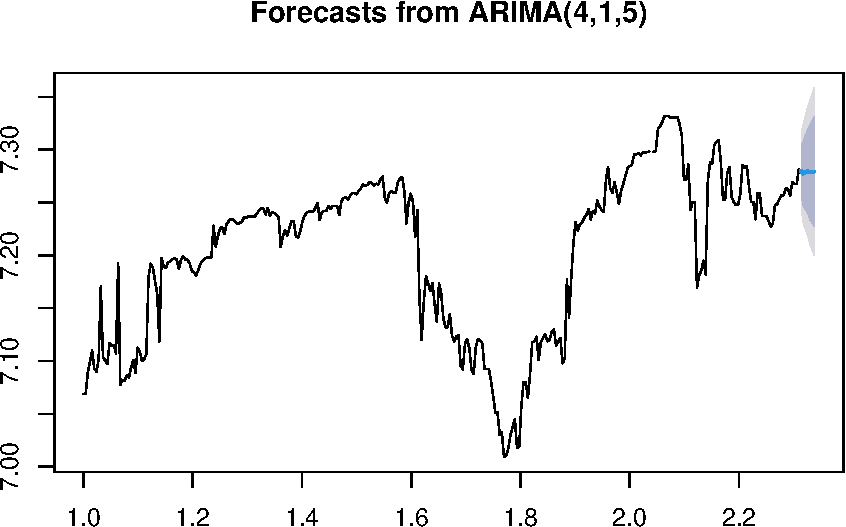
\includegraphics[keepaspectratio]{USD_CNY_Forecast_Report_files/figure-latex/unnamed-chunk-2-1.pdf}}

The shaded area in the plot represents the \textbf{95\% confidence
interval}, indicating the range of uncertainty associated with the
forecast.

\begin{center}\rule{0.5\linewidth}{0.5pt}\end{center}

\subsubsection{Conclusion}\label{conclusion-1}

According to the ARIMA(4,1,5) model, the expected USD/CNY exchange rate
on \textbf{April 16, 2025} is \textbf{7.2793}. This prediction is
consistent with the direction suggested by UIP and CIP models,
indicating a slight \textbf{depreciation of the Chinese yuan} relative
to the U.S. dollar in the short term. Unlike UIP and CIP, the ARIMA
model does not rely on interest rate differentials but purely on
historical price patterns and volatility structure.

\subsection{Comparison of Forecasting
Methods}\label{comparison-of-forecasting-methods}

This section presents a comparative summary of the three forecasting
approaches used to estimate the USD/CNY exchange rate on \textbf{April
16, 2025}.

\subsubsection{Methodological Overview}\label{methodological-overview}

\begin{itemize}
\item
  \textbf{Uncovered Interest Parity (UIP):} Assumes that expected
  returns on domestic and foreign assets are equal in equilibrium. It
  uses interest rate differentials to project the expected future spot
  rate without accounting for currency risk.
\item
  \textbf{Covered Interest Parity (CIP):} Incorporates hedging via
  forward contracts, removing exchange rate risk entirely. The forward
  rate is inferred based on the interest rate differential, assuming no
  arbitrage.
\item
  \textbf{ARIMA Model:} A purely statistical, time-series model that
  relies on the historical behavior of the exchange rate, capturing
  trends and volatility without requiring macroeconomic inputs.
\end{itemize}

\begin{center}\rule{0.5\linewidth}{0.5pt}\end{center}

\subsubsection{Forecasted Exchange
Rates}\label{forecasted-exchange-rates}

\begin{Shaded}
\begin{Highlighting}[]
\NormalTok{ForecastedExchangeRates }\OtherTok{\textless{}{-}} \FunctionTok{tibble}\NormalTok{(}
  \AttributeTok{Method =} \FunctionTok{c}\NormalTok{(}\StringTok{"UIP"}\NormalTok{, }\StringTok{"CIP"}\NormalTok{, }\StringTok{"ARIMA"}\NormalTok{),}
  \StringTok{\textasciigrave{}}\AttributeTok{Forecasted USD/CNY}\StringTok{\textasciigrave{}} \OtherTok{=} \FunctionTok{c}\NormalTok{(uip\_forecast, cip\_forward\_rate, arima\_forecast)}
\NormalTok{)}
\FunctionTok{kable}\NormalTok{(ForecastedExchangeRates)}
\end{Highlighting}
\end{Shaded}

\begin{longtable}[]{@{}lr@{}}
\toprule\noalign{}
Method & Forecasted USD/CNY \\
\midrule\noalign{}
\endhead
\bottomrule\noalign{}
\endlastfoot
UIP & 7.281438 \\
CIP & 7.281438 \\
ARIMA & 7.279264 \\
\end{longtable}

\begin{center}\rule{0.5\linewidth}{0.5pt}\end{center}

\subsubsection{Key Insights and
Conclusions}\label{key-insights-and-conclusions}

\begin{itemize}
\tightlist
\item
  All three models converge on a \textbf{similar forecast} for the
  exchange rate, falling within a narrow range around \textbf{7.28}.
\item
  Both UIP and CIP models yield identical predictions due to the use of
  the same interest rate inputs and short-term horizon. This reinforces
  the theoretical consistency between the two under efficient market
  assumptions.
\item
  The ARIMA model arrives at a slightly lower rate, indicating that
  recent historical dynamics may suggest \textbf{a slightly slower pace
  of yuan depreciation} than what is implied by interest rate
  differentials alone.
\item
  The overall consensus among models is that the \textbf{Chinese yuan is
  likely to experience mild depreciation} against the U.S. dollar over
  the next week, driven primarily by the persistent interest rate
  advantage of the United States.
\end{itemize}

This triangulation across fundamentally different models enhances the
credibility of the forecast and provides a robust basis for short-term
policy or investment decisions.

\end{document}
